\section{Testy wydajnościowe}



\subsection{Test 1}

Pierwszym przypadkiem testowym będzie sprawdzenie czasów znajdowania pierwiastków dla takich wielomianów, których wszystkie współczynniki są równe $1$. W tym miejscu warto wspomnieć, że wielomiany, których większość współczynników jest niezerowa nazywami gęstymi.

Testowane wielomiany można przedstawić wzorem: \\
$W(x) = x^k + x^{k-1} + x^{k-2} + ... + x^2 + x + 1$, gdzie $k$ jest stopniem wielomianu $W$.

\subsubsection{Wielomiany stopnia parzystego}

W przypadku, gdy stopień wielomianu jest liczbą parzystą, a jego wszystkie współczynniki są równe $1$, wielomian nie posiada pierwiastków rzeczywistych. Sprawdźmy ile czasu zajmie każdej ze struktur stwierdzenie o braku pierwiastków rzeczywistych dla wielomianów powyższej postaci.

\begin{table}[H]
	\begin{tabular}{ |p{4cm}|p{2.75cm}|p{2.75cm}|p{3.5cm}|} 
		\hline
		Testowany wielomian & Czas dla PolynomialMap [s] & Czas dla PolynomialVector [s] & Współczynnik czasów \\
		\hline
		$W(x) = x^{10} + x^9 + ... + x + 1$ & 0.077 & 0.079 & 1.026 \\
		$W(x) = x^{20} + x^{19} + ... + x + 1$ & 0.29 & 0.291 & 1.003 \\
		$W(x) = x^{40} + x^{39} + ... + x + 1$ & 1.176 & 1.174 & 0.998 \\
		$W(x) = x^{80} + x^{79} + ... + x + 1$ & 5.046 & 5.048 & 1 \\
		$W(x) = x^{160} + x^{159} + ... + x + 1$  & 22.879 & 23.047 & 1.007 \\
		$W(x) = x^{320} + x^{319} + ... + x + 1$  & 114.311 & 114.382 & 1.001 \\
		\hline
	\end{tabular}
	\caption{Porównanie czasów znajdowania pierwiastków dla gęstych wielomianów parzystego stopnia}
\end{table}

\begin{figure}[H]
	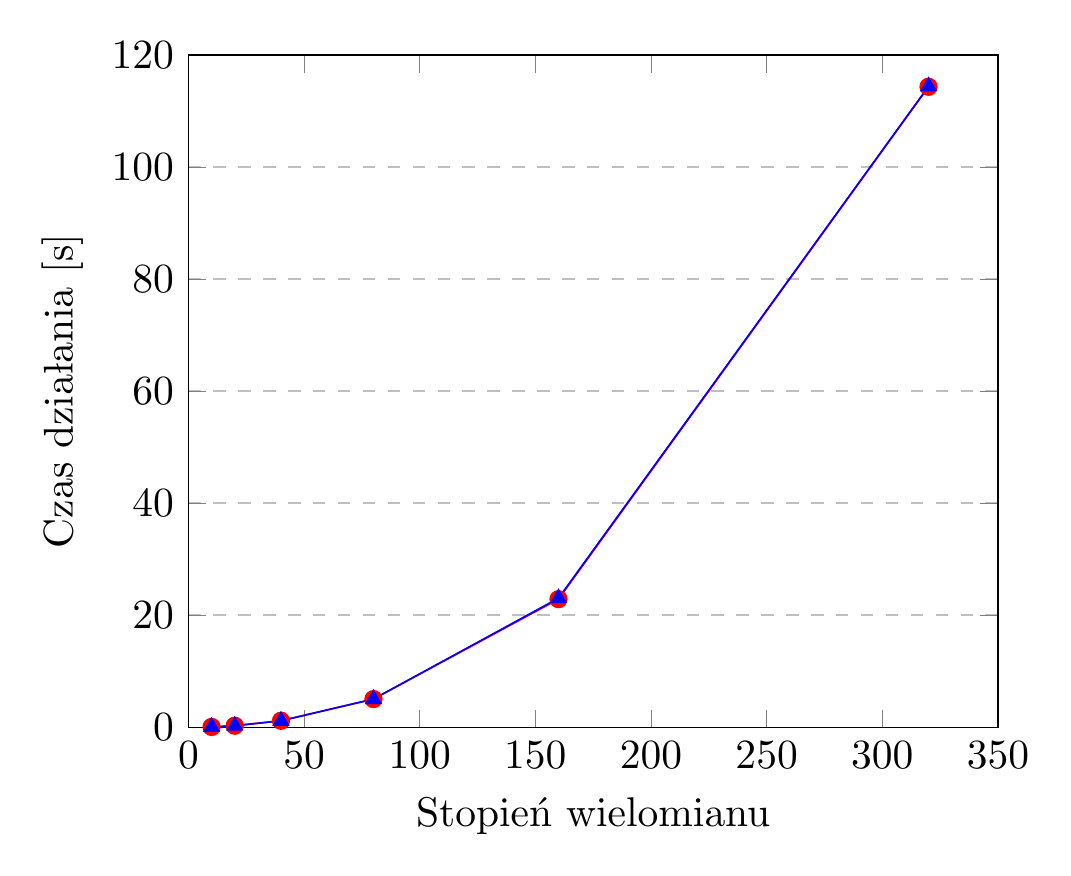
\begin{tikzpicture}[scale=1.5]
	\begin{axis}[
	xlabel={Stopień wielomianu},
	ylabel={Czas działania [s]},
	xmin=0,xmax=350,
	ymin=0,ymax=120,
	ymajorgrids=true,grid style=dashed
	]
	
	\addplot[color=red,mark=*]
	coordinates {
		(10, 0.077)
		(20, 0.29)
		(40, 1.176)
		(80, 5.046)
		(160, 22.879)
		(320, 114.311)
	};
	
	\addplot[color=blue,mark=triangle*]
	coordinates {
		(10, 0.079)
		(20, 0.291)
		(40, 1.174)
		(80, 5.048)
		(160, 23.047)
		(320, 114.382)	
	};
	
	\end{axis}
	\end{tikzpicture}
	\caption{Czasy znajdowania pierwiastków dla gęstych wielomianów parzystego stopnia}
\end{figure}

\subsubsection{Wielomiany stopnia nieparzystego}

To analogiczny test w porównaniu z poprzednim, jednak w tym przypadku stopień wielomianu jest nieparzysty. Wpływa to na liczbę pierwiastków rzeczywistych wielomianu, zwiększając ją o $1$. Sprawdźmy, czy wyniki będą podobne do tych uzyskanych dla wielomianów stopnia parzystego.

\begin{table}[H]
	\begin{tabular}{ |p{4cm}|p{2.75cm}|p{2.75cm}|p{3.5cm}|} 
		\hline
		Testowany wielomian & Czas dla PolynomialMap [s] & Czas dla PolynomialVector [s] & Współczynnik czasów \\
		\hline
		$W(x) = x^{11} + x^{10} + ... + x + 1$ & 3.224 & 3.269 & 1 \\
		$W(x) = x^{21} + x^{20} + ... + x + 1$ & 13.384 & 13.548 & 1 \\
		$W(x) = x^{41} + x^{40} + ... + x + 1$ & 57.336 & 57.336 & 0 \\
		$W(x) = x^{81} + x^{80} + ... + x + 1$ & 260.175 & 261.915 & 1 \\
		$W(x) = x^{161} + x^{160} + ... + x + 1$  & 1286.409 & 1286.261 & 1.002 \\
		$W(x) = x^{321} + x^{320} + ... + x + 1$  & 7190.234 & 7205.386 & 1 \\
		\hline
	\end{tabular}
	\caption{Porównanie czasów znajdowania pierwiastków dla gęstych wielomianów nieparzystego stopnia}
\end{table}

\begin{figure}[H]
	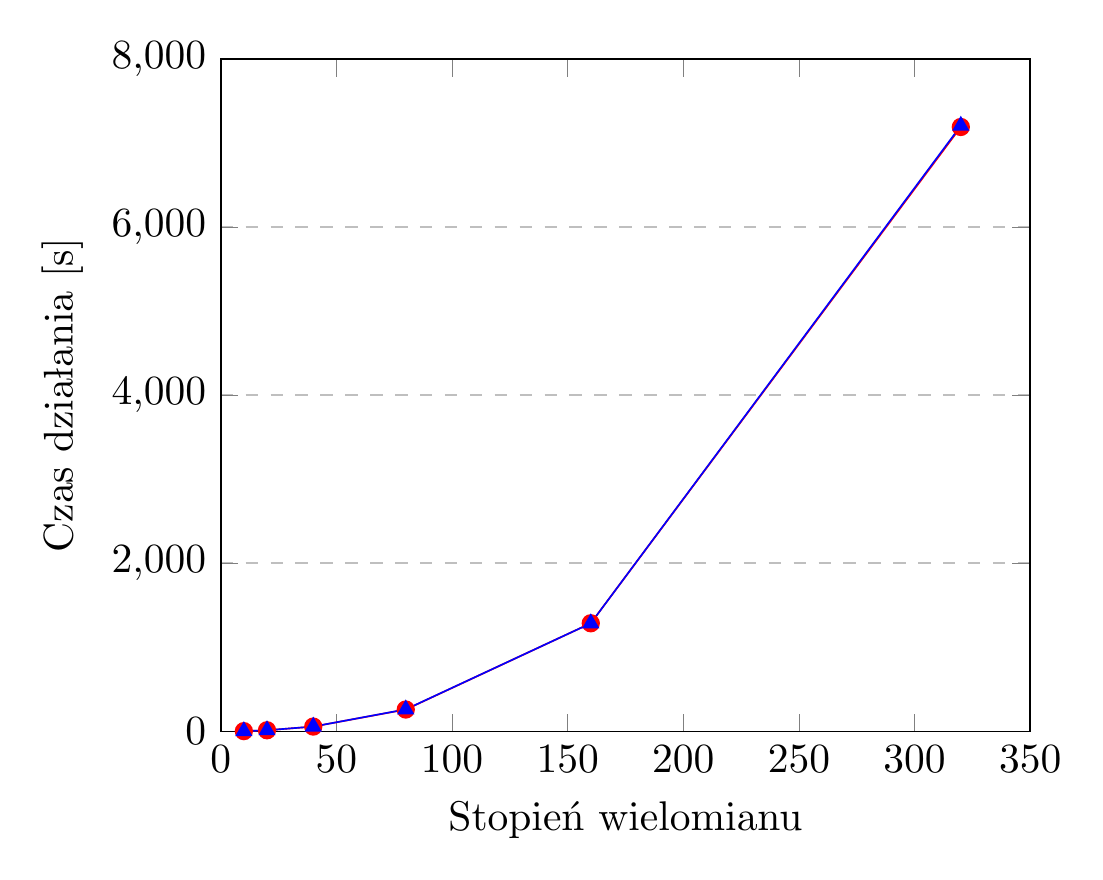
\begin{tikzpicture}[scale=1.5]
	\begin{axis}[
	xlabel={Stopień wielomianu},
	ylabel={Czas działania [s]},
	xmin=0,xmax=350,
	ymin=0,ymax=8000,
	ymajorgrids=true,grid style=dashed
	]
	
	\addplot[color=red,mark=*]
	coordinates {
		(10, 3.224)
		(20, 13.384)
		(40, 57.336)
		(80, 260.175)
		(160, 1286.409)
		(320, 7190.234)
	};
	
	\addplot[color=blue,mark=triangle*]
	coordinates {
		(10, 3.269)
		(20, 13.548)
		(40, 57.336)
		(80, 261.915)
		(160, 1286.261)
		(320, 7205.386)	
	};
	
	\end{axis}
	\end{tikzpicture}
	\caption{Czas znajdowania pierwiastków dla wielomianów zawierających kolejne pierwiastki całkowite}
\end{figure}

\subsection{Wielomiany o losowych współczynnikach}

Test zakłada, że wszystkie współczynniki wielomianu danego stopnia zostaną dobre w sposób losowy. Jako możliwe wartości kolejnych współczynników ustaliłem wszystkie liczby całkowite z przedziału $(-100, 100)$. Oba typy wielomianów zostały przetestowane dla dokładnie tych samych wartości współczynników.

Aby zapewnić reprezentatywność wyników dla danego stopnia wielomianu dla każdego stopnia zostaną stworzony trzy wielomiany. Dla uzyskanych rezultatów zostanie policzona średnia ważona. Zabieg taki pozwoli na uniezależnienie się od skrajnych wyników w generowanie współczynników wielomianu i zwiększy szanse na zaobserwowanie w nich ewentualnej prawidłowości.

